\chapter{细胞呼吸与发酵}\label{ch:g12:respiration-fermentation}

马拉松运动员的肌肉在三个半小时内，
每分钟约消耗半摩尔 \omterm{def:g12:respiration-fermentation:atp}{ATP}——相当于四分之一千克的
这种分子，被成千上万次地生成、利用与再生，所依赖的
储备仅够维持五秒。这些 \omterm{def:g12:respiration-fermentation:atp}{ATP} 分子中的每一个，都要
由一分子葡萄糖或脂肪酸经逐个原子拆解来供能，并需一个
起始时吸入、末尾以水的形式生成的氧分子参与。
\cref{ch:g10:cell-metabolism}已给出物质与能量的总体平衡；
本章打开\omterm{def:g10:cells-common-unit:organelle}{线粒体}，追踪葡萄糖经过
三个阶段，把其中的能量转化为 \omterm{def:g12:respiration-fermentation:atp}{ATP}——并
说明\omterm{def:g10:cells-common-unit:cell}{细胞}在氧气耗尽时如何应对。

\section{ATP：能量通货}

\begin{definition}[ATP]\label{def:g12:respiration-fermentation:atp}
\emph{ATP}\index{ATP}（腺苷三磷酸）是一种\omterm{def:g10:universal-dna:nucleotide}{核苷酸}，
其上依次连有三个磷酸基团。去掉末端一个
磷酸基团，在\omterm{def:g10:cells-common-unit:cell}{细胞}条件下每摩尔释放约\qty{30}{kJ}，而\omterm{def:g10:cells-common-unit:cell}{细胞}的每一个
需能过程——如收缩、运输、
合成，以及萤火虫发光——都由这一去除反应驱动。
产物 ADP 借助本章所述的反应
重新合成为 ATP。\omterm{def:g10:cells-common-unit:cell}{细胞}仅储存数秒用量的 ATP，并持续周转；
静息的人一天之内循环利用的 ATP 约
相当于其自身体重的量。
\end{definition}

\begin{proposition}[能量藏于何处]\label{prop:g12:respiration-fermentation:oxidation}
葡萄糖将能量储存于其碳–氢键中；释放能量
意味着将氢及其电子转移给氧——
即葡萄糖被氧化为二氧化碳，氧被还原为
水。若一步完成，如同火焰中的燃烧，能量将以
热的形式散失。\omterm{def:g10:cells-common-unit:cell}{细胞}则将其分为数十个小步骤，每步
由一种酶催化，并在其中数步捕获部分能量：
氢首先被装载到载体分子上——\emph{还原型
NAD}，只在最后才交给氧。
\end{proposition}
\admitted

\section{三个阶段}

\begin{proposition}[糖酵解]\label{prop:g12:respiration-fermentation:glycolysis}
在\omterm{def:g10:cells-common-unit:cell}{细胞质}中、无氧条件下，一分子葡萄糖（六个碳）
经十步酶促反应分解为两分子\emph{丙酮酸}（每分子三个碳），
这一过程称为\emph{糖酵解}\index{糖酵解}。总账：起始消耗两个
\omterm{def:g12:respiration-fermentation:atp}{ATP}，共产生四个，净增 2 个 \omterm{def:g12:respiration-fermentation:atp}{ATP}，同时
获得两分子携带氢的还原型 NAD。丙酮酸仍保留着
葡萄糖的大部分能量。
\end{proposition}
\admitted

\begin{proposition}[线粒体完成氧化]\label{prop:g12:respiration-fermentation:mitochondrion}
有氧时，丙酮酸进入\emph{线粒体}\index{线粒体}，
这是一种由两层膜包围的\omterm{def:g10:cells-common-unit:organelle}{细胞器}，内膜向内折叠成
\emph{嵴}，包围着液态的\emph{基质}。
\begin{itemize}
  \item 在基质中，每分子丙酮酸经一系列
        反应被分解，即\emph{克雷布斯循环}\index{克雷布斯循环}：其
        三个碳以三分子 $\mathrm{CO_2}$ 的形式离去，其氢
        被装载到载体上（还原型 NAD 及另一种载体），并
        直接生成少量 \omterm{def:g12:respiration-fermentation:atp}{ATP}——每分子丙酮酸一个。
  \item 在内膜上，所载的载体将其
        电子传递给一系列\omterm{def:g11:gene-expression:protein}{蛋白质}，即\emph{呼吸
        链}，电子沿链传递给氧，氧与
        质子结合生成水。沿链释放的能量
        将质子泵过膜，质子经一种旋转
        酶回流，驱动 \omterm{def:g12:respiration-fermentation:atp}{ATP} 的合成——每个葡萄糖约
        26 个。
\end{itemize}
一分子葡萄糖总计约 30 个 \omterm{def:g12:respiration-fermentation:atp}{ATP}（\omterm{prop:g12:respiration-fermentation:glycolysis}{糖酵解} 2 个，
循环 2 个，呼吸链约 26 个），释放六分子 $\mathrm{CO_2}$，消耗六
分子 $\mathrm{O_2}$，其余 \qty{2870}{kJ} 以热的形式散失。
\end{proposition}
\begin{proof}[证据]
将分离的\omterm{def:g10:cells-common-unit:organelle}{线粒体}置于装有氧探针的密闭小室中，
加入葡萄糖时不耗氧，而加入丙酮酸时
则迅速耗氧——\omterm{def:g10:cells-common-unit:organelle}{线粒体}不能从葡萄糖起始，
\omterm{def:g10:cells-common-unit:cell}{细胞质}必须完成此步。加入呼吸链的一种毒物（氰化物）
会立即使耗氧停止，无论存在何种\omterm{def:g11:enzymes-and-phenotype:enzyme}{底物}。加入
ADP 会加快耗氧，而其耗尽则使之减慢：耗氧与 \omterm{def:g12:respiration-fermentation:atp}{ATP} 合成
相偶联。此外，蜂鸟飞行肌和马拉松运动员大腿肌中的
\omterm{def:g10:cells-common-unit:organelle}{线粒体}，其嵴的排列
密度比静息组织中的高出数倍。
\end{proof}

\begin{omfigure}
\begin{tikzpicture}
  \node[anchor=south west, inner sep=0] (img) at (0,0)
    {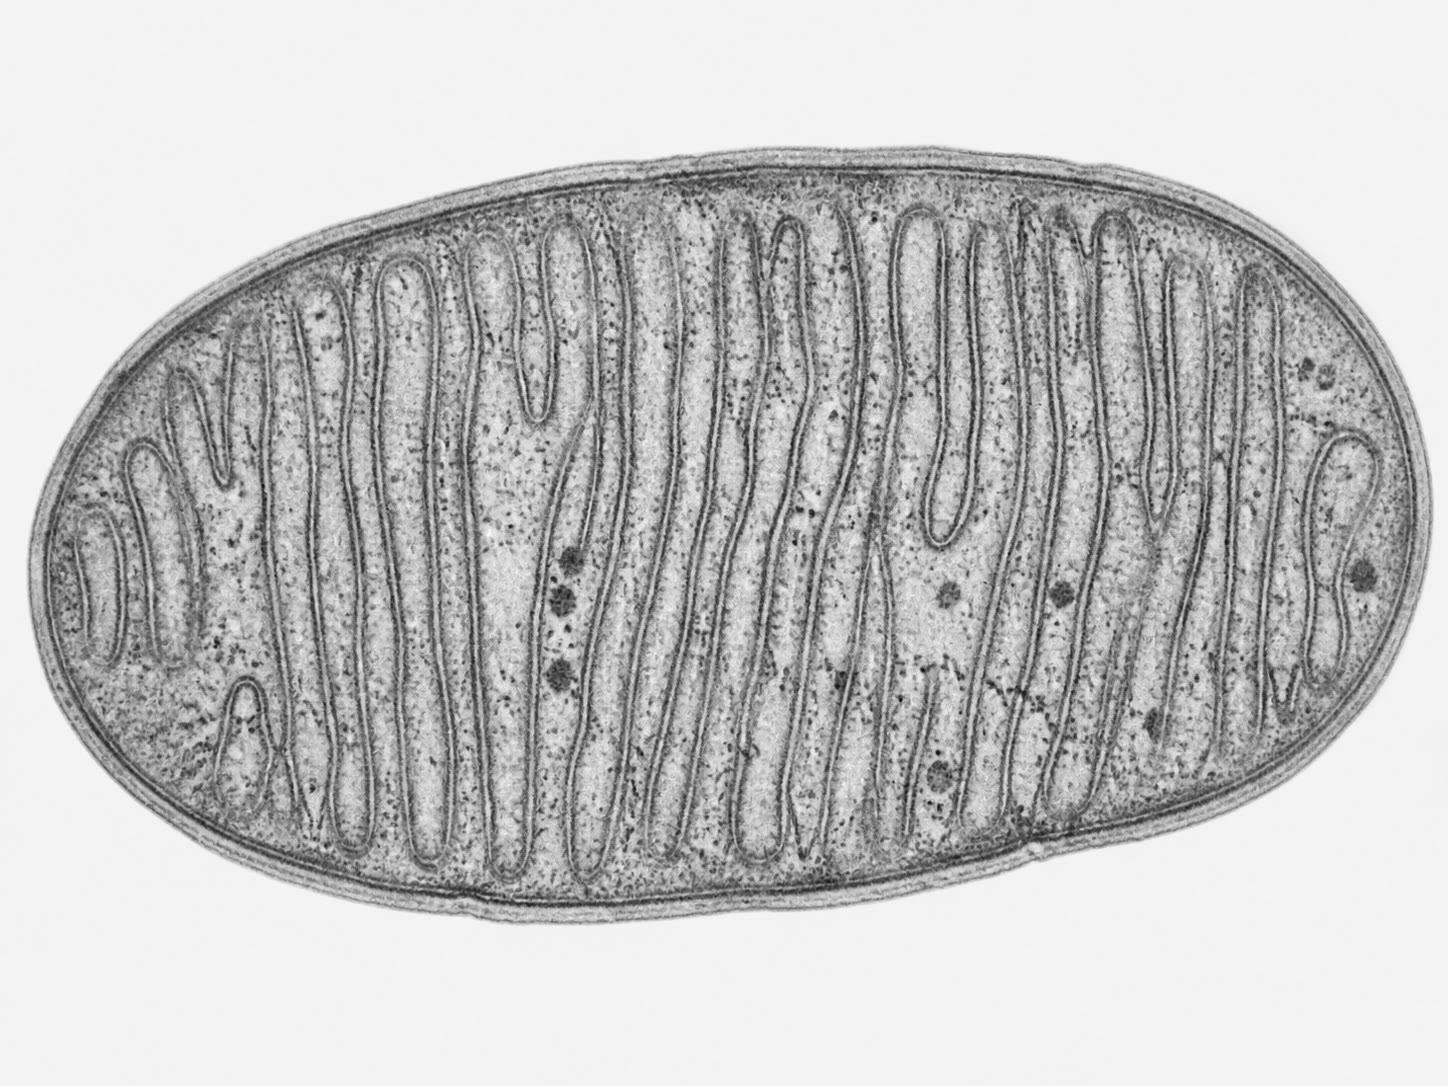
\includegraphics[width=0.5\linewidth]{images/book2/ai/g12-resp-mitochondrion-tem.jpg}};
  \begin{scope}[x={(img.south east)}, y={(img.north west)},
      every node/.style={font=\small}]
    \draw[omDef, thick] (0.08,0.55) -- (-0.04,0.80) node[left, align=right] {外膜};
    \draw[omDef, thick] (0.20,0.45) -- (-0.04,0.25) node[left, align=right] {内膜，\\ 向内折叠成嵴};
    \draw[omDef, thick] (0.55,0.50) -- (0.55,-0.06) node[below] {基质（克雷布斯循环）};
    \draw[omDef, thick] (0.80,0.60) -- (1.04,0.80) node[right, align=left] {嵴：\\ 呼吸链};
  \end{scope}
\end{tikzpicture}

{\small 电子显微镜下的\omterm{def:g10:cells-common-unit:organelle}{线粒体}。内膜
向内折叠成嵴，嵴上携带呼吸链及
\omterm{def:g12:respiration-fermentation:atp}{ATP} 合成酶；嵴之间的液体即基质，进行
\omterm{prop:g12:respiration-fermentation:mitochondrion}{克雷布斯循环}。}
\end{omfigure}

\begin{omfigure}
\begin{tikzpicture}[font=\small, >=Stealth,
  b/.style={draw, rounded corners, align=center, minimum height=0.9cm}]
  % cytoplasm region
  \node[b, fill=omDef!8, minimum width=6.0cm, minimum height=6.2cm] (cyt) at (0,0) {};
  \node[anchor=north, font=\small\bfseries] at (cyt.north) {细胞质};
  \node[b, fill=omMeth!20, text width=2.4cm] (glu) at (0,2.0) {葡萄糖（6 C）};
  \node[b, fill=omProp!20, text width=2.4cm] (pyr) at (0,-0.2) {2 分子丙酮酸 \\（每个 3 C）};
  \draw[->, thick] (glu) -- node[right, align=left, font=\scriptsize] {糖酵解：\\ $+2$ ATP，$+2$ NADH} (pyr);
  \node[b, fill=omThm!15, text width=2.6cm] (ferm) at (0,-2.4) {发酵：\\ 乳酸，或 \\ 乙醇 $+ \mathrm{CO_2}$};
  \draw[->, thick, omThm] (pyr) -- node[right, font=\scriptsize, align=left] {无 $\mathrm{O_2}$：\\ NADH 再生} (ferm);
  % mitochondrion region
  \node[b, fill=omProp!8, minimum width=6.4cm, minimum height=6.2cm, rounded corners=14pt] (mit) at (7.3,0) {};
  \node[anchor=north, font=\small\bfseries] at (mit.north) {线粒体};
  \node[b, fill=omProp!20, text width=2.6cm] (krebs) at (7.3,1.4) {克雷布斯循环 \\ （基质）：\\ 释出 $6\,\mathrm{CO_2}$，\\ $+2$ ATP，载体已装载};
  \node[b, fill=omThm!15, text width=2.8cm] (chain) at (7.3,-1.5) {呼吸链 \\ （内膜）：\\ 载体 $+ \mathrm{O_2} \to \mathrm{H_2O}$，\\ $+26$ ATP};
  \draw[->, thick] (pyr.east) -- node[pos=0.72, above, font=\scriptsize] {有 $\mathrm{O_2}$} (krebs.west |- pyr.east);
  \draw[->, thick] (krebs) -- node[right, font=\scriptsize] {还原型 NAD} (chain);
  \draw[->, thick] (10.9,-1.1) -- (chain.east |- 0,-1.1) node[pos=0, right] {$6\,\mathrm{O_2}$};
  \draw[->, thick] (chain.east |- 0,-1.9) -- (10.9,-1.9) node[right] {$6\,\mathrm{H_2O}$};
  \draw[->, thick] (krebs.east |- 0,1.8) -- (10.9,1.8) node[right] {$6\,\mathrm{CO_2}$};
\end{tikzpicture}

{\small 呼吸作用的三个阶段，以及\omterm{def:g10:cell-metabolism:fermentation}{发酵}这一
捷径。\omterm{def:g10:cells-common-unit:cell}{细胞质}中的\omterm{prop:g12:respiration-fermentation:glycolysis}{糖酵解}产生 2 个 \omterm{def:g12:respiration-fermentation:atp}{ATP} 和 2 个
丙酮酸；在\omterm{def:g10:cells-common-unit:organelle}{线粒体}中，\omterm{prop:g12:respiration-fermentation:mitochondrion}{克雷布斯循环}将其分解为二氧化碳，
并装载载体，再由呼吸链卸载，
将电子交给氧，同时产生大部分 \omterm{def:g12:respiration-fermentation:atp}{ATP}。无氧时，丙酮酸
转入\omterm{def:g10:cell-metabolism:fermentation}{发酵}，不再产生 \omterm{def:g12:respiration-fermentation:atp}{ATP}。}
\end{omfigure}

\begin{example}[读取耗氧曲线]\label{ex:g12:respiration-fermentation:trace}
反应室中的离体\omterm{def:g10:cells-common-unit:organelle}{线粒体}：氧气保持在
\qty{8}{mg/L}；加入葡萄糖，无变化；加入丙酮酸，氧气
以每分钟 \qty{0.5}{mg/L} 的速度下降；加入 ADP，下降
速度加快至每分钟 \qty{1.5}{mg/L}，持续一段时间后，回落至
\num{0.5}；加入氰化物，下降停止。这一曲线说明四点：
\omterm{def:g10:cells-common-unit:organelle}{线粒体}需要丙酮酸而非葡萄糖；耗氧与 \omterm{def:g12:respiration-fermentation:atp}{ATP} 合成
相耦联，这种耦联经由氰化物所阻断的呼吸链实现；
\omterm{def:g10:cells-common-unit:organelle}{线粒体}无事可做时便处于空转状态。
\end{example}

\begin{omfigure}
\begin{tikzpicture}
\begin{axis}[
  width=0.9\linewidth, height=5.6cm,
  axis x line=bottom, axis y line=left,
  xmin=0, xmax=16, ymin=0, ymax=10,
  xlabel={时间（分钟）}, ylabel={溶解 $\mathrm{O_2}$（mg/L）},
  xlabel style={font=\small, at={(axis description cs:0.5,-0.12)}, anchor=north},
  ylabel style={font=\small},
  tick label style={font=\small}, xtick={0,2,4,6,8,10,12,14,16}, ytick={0,2,4,6,8},
  clip=false,
]
\addplot[thick, omThm] coordinates {(0,8) (2,8) (4,8) (6,7) (8,4) (10,3) (12,2) (14,2) (16,2)};
\draw[->, thick] (axis cs:2,9.6) -- (axis cs:2,8.4);
\node[font=\scriptsize, anchor=south] at (axis cs:2,9.7) {葡萄糖};
\draw[->, thick] (axis cs:4,9.6) -- (axis cs:4,8.4);
\node[font=\scriptsize, anchor=south] at (axis cs:4,9.7) {丙酮酸};
\draw[->, thick] (axis cs:6,9.6) -- (axis cs:6,8.4);
\node[font=\scriptsize, anchor=south] at (axis cs:6,9.7) {ADP};
\draw[->, thick] (axis cs:12,9.6) -- (axis cs:12,8.4);
\node[font=\scriptsize, anchor=south] at (axis cs:12,9.7) {氰化物};
\end{axis}
\end{tikzpicture}

{\small 离体\omterm{def:g10:cells-common-unit:organelle}{线粒体}的耗氧量。葡萄糖
无作用；丙酮酸启动耗氧；ADP 加快耗氧，直至
ADP 耗尽；氰化物阻断呼吸链，使耗氧停止。}
\end{omfigure}

\section{无氧条件：发酵}

\begin{proposition}[发酵使载体再生]\label{prop:g12:respiration-fermentation:fermentation}
\omterm{prop:g12:respiration-fermentation:glycolysis}{糖酵解}每分子葡萄糖装载两个 NAD 载体；有氧时，
\omterm{def:g10:cells-common-unit:organelle}{线粒体}将其卸载。无氧时，载体将全部
在数秒内装满，\omterm{prop:g12:respiration-fermentation:glycolysis}{糖酵解}随之停止。\emph{发酵}\index{发酵}
是\omterm{def:g10:cells-common-unit:cell}{细胞质}中卸载载体的方式：丙酮酸本身接受
氢，转变为\emph{乳酸}（肌\omterm{def:g10:cells-common-unit:cell}{细胞}、乳酸
菌），或失去一分子 $\mathrm{CO_2}$ 后转变为\emph{乙醇}（酵母）。
不再产生 \omterm{def:g12:respiration-fermentation:atp}{ATP}；产量仅为\omterm{prop:g12:respiration-fermentation:glycolysis}{糖酵解}的 2 个 \omterm{def:g12:respiration-fermentation:atp}{ATP}，
约为呼吸作用的十五分之一，而产物——乳酸或
乙醇——仍保留葡萄糖的大部分能量。
\end{proposition}
\admitted

\begin{omfigure}
\begin{tikzpicture}
\begin{axis}[
  ybar, bar width=22pt,
  width=0.7\linewidth, height=5.2cm,
  axis x line=bottom, axis y line=left,
  ymin=0, ymax=36, ylabel={每分子葡萄糖的 ATP 数},
  ylabel style={font=\small},
  symbolic x coords={fermentation, glycolysis + Krebs, full respiration},
  xtick=data, xticklabels={发酵, 糖酵解 + 克雷布斯循环, 完整呼吸}, tick label style={font=\small},
  enlarge x limits=0.3, ytick={0,10,20,30},
  nodes near coords, nodes near coords style={font=\small},
]
\addplot[fill=omThm!45, draw=omThm] coordinates {(fermentation,2) (glycolysis + Krebs,4) (full respiration,30)};
\end{axis}
\end{tikzpicture}

{\small 每分子葡萄糖的 \omterm{def:g12:respiration-fermentation:atp}{ATP} 产量。仅\omterm{prop:g12:respiration-fermentation:glycolysis}{糖酵解}（配以
使载体再生的\omterm{def:g10:cell-metabolism:fermentation}{发酵}）得 2 个；\omterm{prop:g12:respiration-fermentation:mitochondrion}{克雷布斯循环}直接
增加 2 个；需氧的呼吸链再增加其余 26 个。}
\end{omfigure}

\begin{example}[肌肉的选择]\label{ex:g12:respiration-fermentation:muscle}
短跑运动员的\omterm{def:g10:muscles-and-joints:muscle}{肌纤维}所需 \omterm{def:g12:respiration-fermentation:atp}{ATP} 的速度快于\omterm{def:g10:cells-common-unit:organelle}{线粒体}和
氧气供应所能提供的速度；乳酸\omterm{def:g10:cell-metabolism:fermentation}{发酵}的\omterm{prop:g12:respiration-fermentation:glycolysis}{糖酵解}
提供 \omterm{def:g12:respiration-fermentation:atp}{ATP} 的速度快三倍，而葡萄糖消耗为十五倍，
乳酸不断积累，直到疼痛迫使运动停止。马拉松
跑者的\omterm{def:g10:muscles-and-joints:muscle}{肌纤维}依靠呼吸作用供能，速度缓慢，几乎
可持续很长时间，既燃烧葡萄糖也燃烧脂肪；其\omterm{def:g10:cells-common-unit:organelle}{线粒体}
更大、数量更多，毛细血管更密，乳酸含量
始终较低。在\cref{ch:g10:muscles-and-joints}中
所述的\omterm{def:g10:muscles-and-joints:muscle}{肌纤维}类型，正是\omterm{def:g10:cells-common-unit:cell}{细胞}内置的这两种策略。
\end{example}

\begin{method}[能量收支的计算]\label{met:g12:respiration-fermentation:budget}
\begin{enumerate}
  \item 将所需功率换算为 \omterm{def:g12:respiration-fermentation:atp}{ATP}：每摩尔可用 \omterm{def:g12:respiration-fermentation:atp}{ATP} 约 \qty{30}{kJ}，
        则 \qty{1}{kW} 的\omterm{def:g10:cell-metabolism:metabolism}{代谢}功率约合
        每分钟 \qty{2}{mol} 的 \omterm{def:g12:respiration-fermentation:atp}{ATP}。
  \item 将 \omterm{def:g12:respiration-fermentation:atp}{ATP} 换算为燃料：呼吸作用中每分子葡萄糖
        可产 30 个 \omterm{def:g12:respiration-fermentation:atp}{ATP}，\omterm{def:g10:cell-metabolism:fermentation}{发酵}中则为 2 个。
  \item 将燃料换算为氧气：每分子葡萄糖经呼吸作用需 6 $\mathrm{O_2}$，
        每摩尔气体的体积按 \qty{24}{L} 计。
  \item 将所需氧气与血液所能输送的量相比较
        （见\cref{ch:g10:heart-lungs-effort}）：不足部分由
        \omterm{def:g10:cell-metabolism:fermentation}{发酵}及其所产乳酸补足。
\end{enumerate}
\end{method}

\begin{remark}[光合作用的镜像]\label{rem:g12:respiration-fermentation:mirror}
\omterm{def:g10:cell-metabolism:autotrophy}{光合作用}利用光，把电子从水转移到载体上，
再用这些电子将二氧化碳还原为糖，并释放氧气；
呼吸作用则把电子从糖上卸下，交给载体，
再传递给氧气生成水，并释放二氧化碳，同时利用
释放的能量合成 \omterm{def:g12:respiration-fermentation:atp}{ATP}。这两个过程分别由两种\omterm{def:g10:cells-common-unit:organelle}{细胞器}承担，
二者原本都是独立生活的细菌（见\cref{ch:g12:diversification-of-life}），
\omterm{def:g12:photosynthesis:chloroplast}{叶绿体}为\omterm{def:g10:cells-common-unit:organelle}{线粒体}提供其所消耗的物质；二者合作，
将阳光转化为每个\omterm{def:g10:cells-common-unit:cell}{细胞}通用的“能量货币”，而
大气中的氧气正是两者收支相抵的结果。
\end{remark}

\section{练习}

\begin{exercise}[$\star$]\label{exo:g12:respiration-fermentation:1}
\omterm{def:g12:respiration-fermentation:atp}{ATP} 是什么？\omterm{def:g10:cells-common-unit:cell}{细胞}利用它时会发生什么变化？
\end{exercise}

\begin{exercise}[$\star$]\label{exo:g12:respiration-fermentation:2}
写出呼吸作用的三个阶段，说明每个阶段发生的场所，
以及各阶段的产物。
\end{exercise}

\begin{exercise}[$\star$]\label{exo:g12:respiration-fermentation:3}
描述\omterm{def:g10:cells-common-unit:organelle}{线粒体}，并说明呼吸作用的哪个阶段
在其每个区室中进行。
\end{exercise}

\begin{exercise}[$\star$]\label{exo:g12:respiration-fermentation:4}
\omterm{def:g10:cell-metabolism:fermentation}{发酵}对\omterm{def:g10:cells-common-unit:cell}{细胞}有何作用？它能产生什么？
\end{exercise}

\begin{exercise}[$\star$]\label{exo:g12:respiration-fermentation:5}
比较呼吸作用与\omterm{def:g10:cell-metabolism:fermentation}{发酵}的 \omterm{def:g12:respiration-fermentation:atp}{ATP} 产量，以及
两者最终留下的产物。
\end{exercise}

\begin{exercise}[$\star\star$]\label{exo:g12:respiration-fermentation:6}
根据氧气变化曲线，四次加入分别说明了什么？
\end{exercise}

\begin{exercise}[$\star\star$]\label{exo:g12:respiration-fermentation:7}
为什么分离出的\omterm{def:g10:cells-common-unit:organelle}{线粒体}不能利用葡萄糖，而完整的\omterm{def:g10:cells-common-unit:cell}{细胞}却可以？
\end{exercise}

\begin{exercise}[$\star\star$]\label{exo:g12:respiration-fermentation:8}
解释：若不存在\omterm{def:g10:cell-metabolism:fermentation}{发酵}，
无氧时\omterm{prop:g12:respiration-fermentation:glycolysis}{糖酵解}为何会在数秒内停止。
\end{exercise}

\begin{exercise}[$\star\star$]\label{exo:g12:respiration-fermentation:9}
某\omterm{def:g10:cells-common-unit:cell}{细胞}每秒需要 60 个 \omterm{def:g12:respiration-fermentation:atp}{ATP}。
若分别由呼吸作用和\omterm{def:g10:cell-metabolism:fermentation}{发酵}供能，每秒需消耗多少个葡萄糖分子？
\end{exercise}

\begin{exercise}[$\star\star$]\label{exo:g12:respiration-fermentation:10}
氰化物会在数分钟内致命。请从呼吸链的角度解释其原因，
以及脑和心脏为何最先衰竭。
\end{exercise}

\begin{exercise}[$\star\star$]\label{exo:g12:respiration-fermentation:11}
呼出的二氧化碳来自何处，请逐阶段说明，
呼吸作用生成的水又从何而来？
\end{exercise}

\begin{exercise}[$\star\star\star$]\label{exo:g12:respiration-fermentation:12}
肌肉在比赛中产生乳酸，比赛后，肝脏
利用呼吸作用产生的 \omterm{def:g12:respiration-fermentation:atp}{ATP}，将乳酸重新转化为葡萄糖。
试解释，为何全身为肌肉所\omterm{def:g10:cell-metabolism:fermentation}{发酵}的那个葡萄糖
最终付出了多于 30 个 \omterm{def:g12:respiration-fermentation:atp}{ATP} 的代价。
\end{exercise}

\begin{exercise}[$\star\star\star$]\label{exo:g12:respiration-fermentation:13}
酵母在空气中缓慢利用葡萄糖，不产生乙醇；密封时则快速利用葡萄糖并产生乙醇。
请结合产量加以解释，并说明为何面团
无论酵母是否有空气都会膨胀。
\end{exercise}

\begin{exercise}[$\star\star\star$]\label{exo:g12:respiration-fermentation:14}
新生儿的棕色脂肪\omterm{def:g10:cells-common-unit:cell}{细胞}含有\omterm{def:g10:cells-common-unit:organelle}{线粒体}，其呼吸链运行
时不合成 \omterm{def:g12:respiration-fermentation:atp}{ATP}，质子流被短路。这些\omterm{def:g10:cells-common-unit:cell}{细胞}
转而产生什么？这对新生儿有何益处？
\end{exercise}

\begin{exercise}[$\star\star\star$]\label{exo:g12:respiration-fermentation:15}
逐点比较呼吸作用与\omterm{def:g10:cell-metabolism:autotrophy}{光合作用}：电子的来源与去向、
消耗和释放的气体、能量的输入与输出、所在\omterm{def:g10:cells-common-unit:organelle}{细胞器}。
然后用一句话说明，为何二者在地球上
都不能离开对方而存在。
\end{exercise}

\section{问题：每分钟半摩尔 ATP}

\begin{problem}[{周末问题——跑者的能量，从瓦特追踪到分子
：计数 ATP，估算葡萄糖与氧气，
测定线粒体所占的份额，以及呼吸链
无法支付的冲刺}]
\label{pb:g12:respiration-fermentation:1}
跑者维持 \qty{1000}{W} 的\omterm{def:g10:cell-metabolism:metabolism}{代谢}功率，其中约
三分之一以 \omterm{def:g12:respiration-fermentation:atp}{ATP} 形式被捕获，其余以热量散失。取
每摩尔 \omterm{def:g12:respiration-fermentation:atp}{ATP} 可用能量 \qty{30}{kJ}，每分子葡萄糖在
呼吸作用中产 30 个 \omterm{def:g12:respiration-fermentation:atp}{ATP}，\omterm{def:g10:cell-metabolism:fermentation}{发酵}中产 2 个，每摩尔葡萄糖
为 \qty{2870}{kJ}；每摩尔气体 \qty{24}{L}，葡萄糖摩尔质量 \qty{180}{g/mol}。

\medskip
\noindent\textbf{第一部分——\omterm{def:g12:respiration-fermentation:atp}{ATP}。}
\begin{enumerate}
  \item 跑者每分钟消耗多少摩尔 \omterm{def:g12:respiration-fermentation:atp}{ATP}？
        （只计以 \omterm{def:g12:respiration-fermentation:atp}{ATP} 形式被捕获的三分之一。）
  \item 按 \qty{507}{g/mol} 计，这些 \omterm{def:g12:respiration-fermentation:atp}{ATP} 的质量是多少？与
        肌肉任一时刻所储存的几克相比较。
  \item 每个 \omterm{def:g12:respiration-fermentation:atp}{ATP} 分子每分钟被再生多少次，
        若人体的 \omterm{def:g12:respiration-fermentation:atp}{ATP} 储量为 \qty{50}{g}？
  \item 若这些 \omterm{def:g12:respiration-fermentation:atp}{ATP} 全部由呼吸作用产生，
        每分钟需消耗多少摩尔葡萄糖？
  \item 这一过程每分钟需要多少升氧气？
        并与 $\dot V\!\mathrm{O_2}$max 为 \qty{4}{L/min} 相比较。
\end{enumerate}

\medskip
\noindent\textbf{第二部分——\omterm{def:g10:cells-common-unit:organelle}{线粒体}的份额。}
\begin{enumerate}[resume]
  \item 每个葡萄糖产生的 30 个 \omterm{def:g12:respiration-fermentation:atp}{ATP} 中，
        有多少在\omterm{def:g10:cells-common-unit:cell}{细胞质}中生成，有多少在\omterm{def:g10:cells-common-unit:organelle}{线粒体}中生成？
        跑者的 \omterm{def:g12:respiration-fermentation:atp}{ATP} 中，\omterm{def:g10:cells-common-unit:organelle}{线粒体}所占比例是多少？
  \item 她每分钟呼出多少摩尔 $\mathrm{CO_2}$，
        它们分别来自呼吸作用的哪一阶段？
  \item 一个葡萄糖分子所含的 \qty{2870}{kJ} 能量中，有多少转化为 \omterm{def:g12:respiration-fermentation:atp}{ATP}？
        其余的能量去了哪里？跑者对此又如何应对？
  \item 她肌肉\omterm{def:g10:cells-common-unit:organelle}{线粒体}的内膜总面积约为
        \qty{1000}{m^2}。呼吸链为何需要如此大的表面积？
  \item 训练使她\omterm{def:g10:muscles-and-joints:muscle}{肌纤维}中的\omterm{def:g10:cells-common-unit:organelle}{线粒体}数量加倍。上述量中，
        哪些因此改变，哪些不变？
\end{enumerate}

\medskip
\noindent\textbf{第三部分——冲刺。}
在最后的冲刺中，她的肌肉需要以 \omterm{def:g12:respiration-fermentation:atp}{ATP} 形式提供功率 \qty{800}{W}，持续
30 秒，而呼吸作用受限于血液所输送的氧气，
至多只能以 \omterm{def:g12:respiration-fermentation:atp}{ATP} 形式供应 \qty{400}{W}。
\begin{enumerate}[resume]
  \item 冲刺过程共需多少摩尔 \omterm{def:g12:respiration-fermentation:atp}{ATP}？
  \item 呼吸作用在 30 秒内能提供其中多少，
        其余多少必须由\omterm{def:g10:cell-metabolism:fermentation}{发酵}提供？
  \item \omterm{def:g10:cell-metabolism:fermentation}{发酵}部分消耗多少摩尔葡萄糖，
        并生成多少摩尔乳酸？
  \item 比较冲刺过程中两条途径每生成一个 \omterm{def:g12:respiration-fermentation:atp}{ATP} 所消耗的葡萄糖，
        肌肉为何能接受这种浪费？
  \item 比赛结束后，乳酸会被氧化，或转化回
        葡萄糖。试解释她停止运动后，耗氧量为何
        在数分钟内仍保持较高水平。
\end{enumerate}

\medskip
\noindent\textbf{第四部分——另一种燃料。}
脂肪每克提供约 \qty{38}{kJ} 能量；产生相同能量时，每克脂肪
所需氧气比葡萄糖约多 20\%。
\begin{enumerate}[resume]
  \item 若她一半的 \qty{1000}{W} 功率来自脂肪，
        她每小时将燃烧多少质量的脂肪？
  \item 脂肪虽然每克所含能量更多，但
        为何每升氧气所产生的功率反而更低？
  \item 脂肪酸在\omterm{prop:g12:respiration-fermentation:mitochondrion}{克雷布斯循环}处进入呼吸作用，绕过
        \omterm{prop:g12:respiration-fermentation:glycolysis}{糖酵解}。那么，三个阶段中，脂肪无法利用的是哪一个？
        由此对冲刺有何影响？
  \item 大脑仅依靠葡萄糖供能，为何比赛中
        尽管肌肉正摄取血液中的大部分葡萄糖，
        大脑仍能持续工作？
  \item 请给出结论：跑者每分钟所用 \omterm{def:g12:respiration-fermentation:atp}{ATP} 的摩尔数、
        支付这些 \omterm{def:g12:respiration-fermentation:atp}{ATP} 所需的氧气升数，以及
        产生其中大部分 \omterm{def:g12:respiration-fermentation:atp}{ATP} 的呼吸作用阶段。
\end{enumerate}
\end{problem}
